\documentclass[tikz, border=2mm]{standalone}
\usepackage{tikz}
\usepackage{amsmath}
\usepackage{amsfonts}
\usepackage{amssymb}

\begin{document}
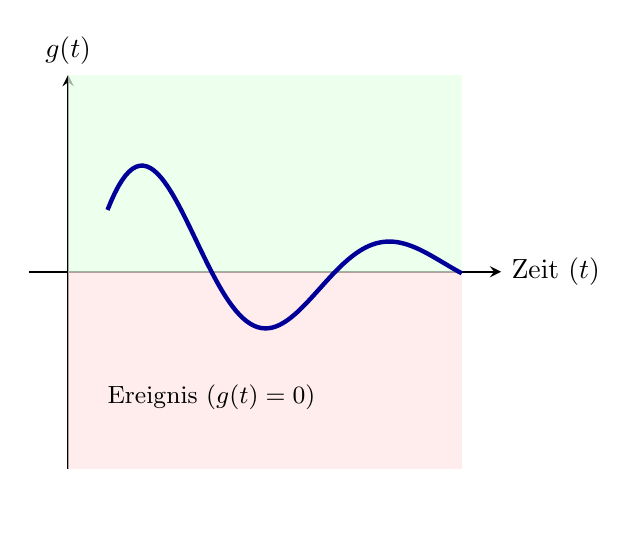
\begin{tikzpicture}[
    >=stealth,
    axis/.style={thick},
    function/.style={ultra thick, blue!60!black},
    zerocrossing/.style={circle, fill=red, inner sep=2pt},
    area_pos/.style={fill=green!10, opacity=0.7},
    area_neg/.style={fill=red!10, opacity=0.7},
    label_style/.style={font=\small}
]

% Define coordinates
\coordinate (origin) at (0,0);
\coordinate (x_end) at (6,0);
\coordinate (y_end_pos) at (0,3);
\coordinate (y_end_neg) at (0,-3);

% Draw axes
\draw[axis, ->] (0, -2.5) -- (0, 2.5) node[above] {$g(t)$};
\draw[axis, ->] (-0.5, 0) -- (5.5, 0) node[right] {Zeit ($t$)};

% Shade areas for sign change
\path[area_pos] (0,0) rectangle (5,2.5);
\path[area_neg] (0,0) rectangle (5,-2.5);

% Draw the function g(t)
\draw[function] plot[domain=0.5:5, samples=100] (\x, {2*exp(-0.4*\x)*sin(deg(2*\x-0.5))});

% Mark the zero-crossing point
% Find approximate zero crossing for sin(2x-0.5) = 0 => 2x-0.5 = pi => 2x = pi+0.5 => x = (pi+0.5)/2 approx 1.82
\draw[zerocrossing] (1.82, 0) node[below=5pt, label_style] {Ereignis ($g(t)=0$)};

\end{tikzpicture}
\end{document}
